\begin{figure}
	\centering
	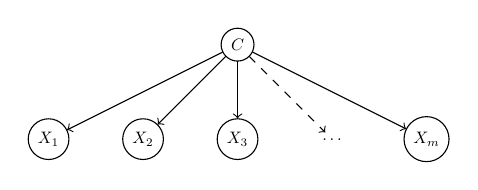
\begin{tikzpicture}[
		scale=0.6,
		every node/.style={scale=0.6}
	]

		\node[circle,draw=black] (C) at (0,2) {$C$};
		\node[circle,draw=black] (X1) at (-4,0) {$X_1$};
		\node[circle,draw=black] (X2) at (-2,0) {$X_2$};
		\node[circle,draw=black] (X3) at (0,0) {$X_3$};
		\node (Xi) at (2,0) {$\dots$};
		\node[circle,draw=black] (Xm) at (4,0) {$X_m$};
		\draw[->] (C) -- (X1);
		\draw[->] (C) -- (X2);
		\draw[->] (C) -- (X3);
		\draw[->,dashed] (C) -- (Xi);
		\draw[->] (C) -- (Xm);
		
	\end{tikzpicture}
\end{figure}